\chapter{Implementation}
\label{cha:implementation}

This chapter provides the reader understanding of the project organisation, architecture and algorithms used.

\begin{figure}[!ht]
	\centering
	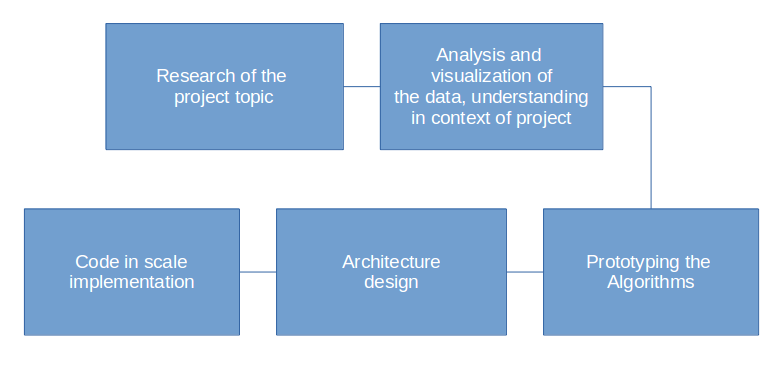
\includegraphics[width=0.6\textwidth]{images/workflow.png}\\
	\caption{ Project workflow }
	\label{fig:workflow}
\end{figure}
\FloatBarrier

At first, we researched the topic of LBS, stop detection, clustering and graph theory. Second step was to understand the data, start prototyping the algorithm for stop detection and visualize. Third step was to build four independent components using Apache Spark API and Scala - stop detection algorithm, clustering, graph analysis and web server. Fourth step was to build a scalable architecture and mock additional 3rdparty components (Minio S3 and Apache Spark containers).

\section{Scripts for data analysis in python and QGIS}

To understand the data we have used a set of tools in python \cite{pythonQgis}. These enabled us to quickly understand the data in general (nubmer of users, avarage number of points, average duration, distance, speed etc) and per user (plotting distances and speeds between points in time). We also extensively used a tool called QGIS in order to visualize data on the map. 

\section{Architecture - batch processing in Apache Spark}

The architecture of the project follows an elegant microservice concept, using independent deployable components.
The project primarily consists of three independent components; S3 storage (a protocol for data storage, in this case open source \textit{Minio} in Docker container), Apache Spark cluster (distributed compute engine over nodes), and a web server with spark jobs and spark-submit. See figure \ref{fig:architect}.

\begin{figure}[!ht]
	\centering
	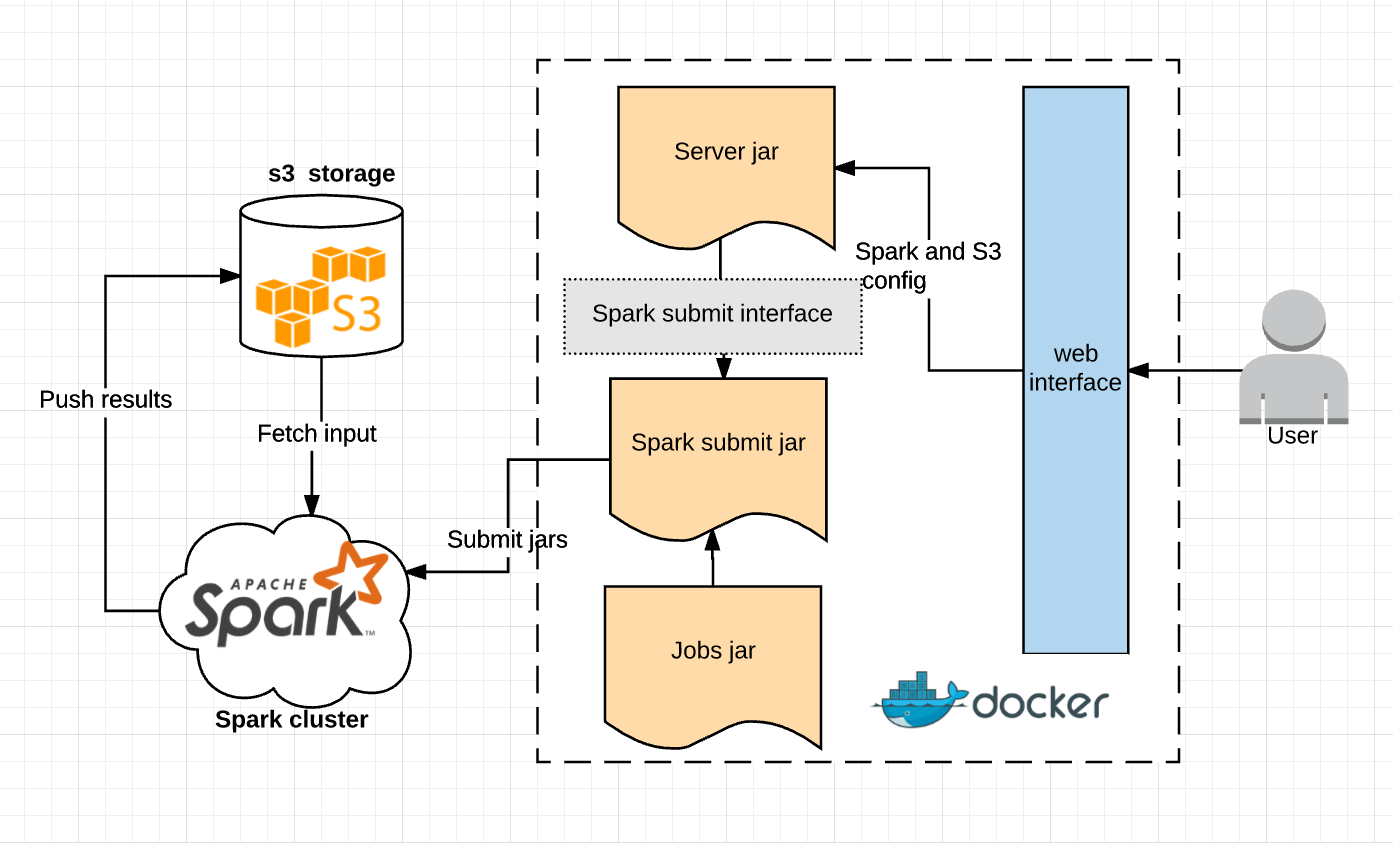
\includegraphics[width=0.8\textwidth]{images/architect.png}\\
	\caption{ Architecture of implemented project, using s3, spark, and docker}
	\label{fig:architect}
\end{figure}
\FloatBarrier

The stop detection jobs are bundled in jars and submitted through the \textbf{Spark submit interface} to the \textbf{Apache Spark cluster}. They will there be load balanced over the slaves by the Spark master which fetches the input file from the \textbf{s3 storage}. This storage can be local or deployed on a shared cloud service. After the computation is finished the master can push data back into the \textbf{s3 storage}.

To easily deploy the application and make it environmental agnostic we bundled everything into the container platform Docker. 

Let us describe a basic scenario:

\begin{enumerate}
  \item 
User starts the docker containers which will start spark cluster and s3 storage.
  \item 
User uploads the input file on to the S3 storage.
  \item 
User runs docker container containing the project code (macromovements jobs jar, spark submit jar and web server jar)
  \item 
User accesses the web interface, provide configuration such as the url of the input file (in S3) and the url where the Spark master resides.  
  \item 
User runs the stop detection job from the web interface by pressing the "setup" and "run" buttons. Output will be displayed using Leaflet Javascript library on the map
\end{enumerate}

\section{Determining stop location}
\label{cha:stopdet_impl}

This section discusses implementation details of the algorithm used to identify stops. \autoref{fig:stop_algo} shows block diagram of stop detection algorithm. The input to the algorithm is list of vectors containing at its first 5 elements day of the week, time of day, user id, latitude and longitude of the recorded location. 

\begin{figure}[!ht]
	\centering
	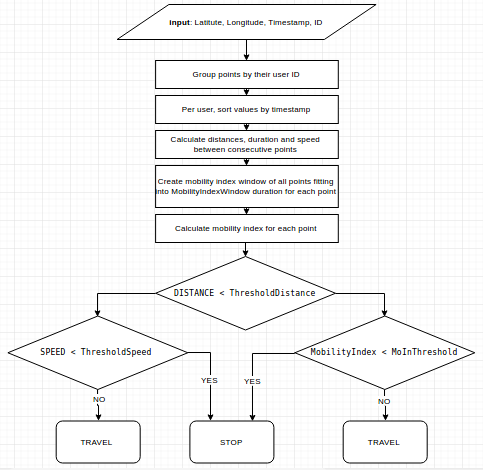
\includegraphics[width=0.95\textwidth]{images/stop_algo.png}
	\caption{ Stop detection algorithm for proactive localization services. }
	\label{fig:stop_algo}
\end{figure} 

\FloatBarrier

The first phase of stop detection algorithm is to group points according to user id. As algorithm is implemented in Spark, each user is processed in parallel. Per user, values are sorted according to their timestamp. Distance, speed and duration is calculated for each consecutive pair of points. Values are being filtered for anomalies in the next step. Mobility Index for each point is calculated, as discussed in \autoref{cha:stopdet_mi}. Further, decision based on thresholds is made whether the point is stop or not. 


\section{Clustering}

%TODO descib in related work
 The implementations of clustering were primarily done by using open source implementations and extending it to our needs. For clustering we used the algorithm DBSCAN. 
 
We wanted a scalable implementation of DBSCAN that could handle large data sets, preferable in parallel. We decided to use Apache Spark, a scalable engine for large-scale data processing \cite{spark}. For this we used an implementation by Irving Cordova, explained in Related work, \ref{cha:relatedwork}. 

Along as using this implementation we extended it with an area version, which divided the data set into predefined boxes. Each box were assign different parameters (discussed in Evaluation, \ref{cha:evaluation} and ran in parallel. After each box was finished the results were merged and written to a file along with important output (such as latitude, longitude, user id, cluster id).

Other versions of DBSCAN were also implemented that ran the jobs in batches and stored it in different files, used for evaluating the results and plotting them in the graph visualization tool QGIS.


\section{Analyzing the user movement graph}
We have used GraphX and Python for creating and analyzing the user movement graph. GraphX was used for creating the data sets and the graph. Before creating the graph, we filtered the data and structured it in a suitable format. 

Filtering was essential at this step as the clustering algorithm identified many stop points as outliers with cluster id=0. We filtered out these outliers from the main data set. With the filtered data, our task was to determine the vertex and edge sets. We used trip count values for each source destination pair as the edge weight. Next task was to create the graph.
 
GraphX provides built-in functions to extract many different properties of a graph. We used GraphX for the indegrees, outdegrees and PageRank values and also NetworkX library of Python to obtain the strongly connected components and betweenness values of our graph. We plotted the results using Python so that we could form a better understanding of the data. It also helped us determine thresholds while calculating top indegree, outdegree, pagerank and betweenness values. We also used the tool QGIS to visualize the property values with respect to physical locations in cities.

\section{User Interface}
To bundle our three parts; stop detection, clustering of detected stop, and graph analysis we developed a web based user interface where job files could be submitted to a running Spark cluster from a specified Amazon S3 storage. The UI was build upon leaflet\cite{leaflet}, a interactive map library for JavaScript, and featured functionality for running the jobs, displaying  the clusters and visualizing graph information such as connected component with out and in degree. To minimize executing time we implemented functionality for displaying previously ran job, instead of re executing jobs it could now display previously ran jobs. When a stop is clicked statistics about the stop appears and lines are drawn on the map according to the out and in degrees (connected travellers to/from this stop to another captured one) See figure \ref{fig:ui_berlin}

The current UI provides following features:
\begin{itemize}
  \item Interactive world \textbf{map} for zooming and panning
  \item \textbf{S3 input file for ETL}: S3 bucket and file name of the input job (currently csv file)  
  \item \textbf{Spark master address}: URL of the spark master that should process the job
  \item \textbf{S3 storage URL}: The URL of the running S3 instance (could be local or public)
  \item \textbf{Test}: Test if job is OK and we can connect to Spark and S3
  \item \textbf{Run}: Run the job and display it on map (in case of a result file, just display the result)
  \item \textbf{Export to CSV}: Download the result output as a csv file for further use, such as not having to re-run the job again. 
  \item \textbf{Statistics about stop}: Panel displaying information  graph information about the clicked cluster, such as id, size, in/out degrees, PageRank etc. 
\end{itemize}

\begin{figure}[!ht]
	\centering
	\includegraphics[width=1\textwidth]{images/ui_berlin.png}\\
	\caption{ Screenshot of the user interface }
	\label{fig:ui_berlin}
\end{figure}
\FloatBarrier
